\documentclass{beamer} 

\usepackage[utf8]{inputenc}
\usepackage[T1]{fontenc}
\usepackage{graphicx}
\usepackage[serbian]{babel}
\usepackage{multicol}
\usepackage{tikz}
\usetikzlibrary{shapes.geometric, arrows}


\usetheme{default}
\begin{document}


% TikZ blok dijagram stilovi
\tikzstyle{block} = [rectangle, rounded corners, minimum width=3cm, minimum height=1cm, text centered, draw=black, fill=blue!30]
\tikzstyle{arrow} = [thick,->,>=stealth]

\title{VertexVoyage: Distribuirani node2vec algoritam za embedovanje čvorova u realnim mrežama - analiza ubrzanja na klasteru sa više čvorova}
\author{Stefan Nožinić \\
Departman za matematiku i informatiku \\
Prirodno-matematički fakultet \\
Univerzitet u Novom Sadu \\
Mentor: \MakeLowercase{dr} Miloš Savić
}
\date{11. septembar 2025.}

\frame{
\titlepage
}

\section{Uvod i motivacija}
\begin{frame}{Uvod}
    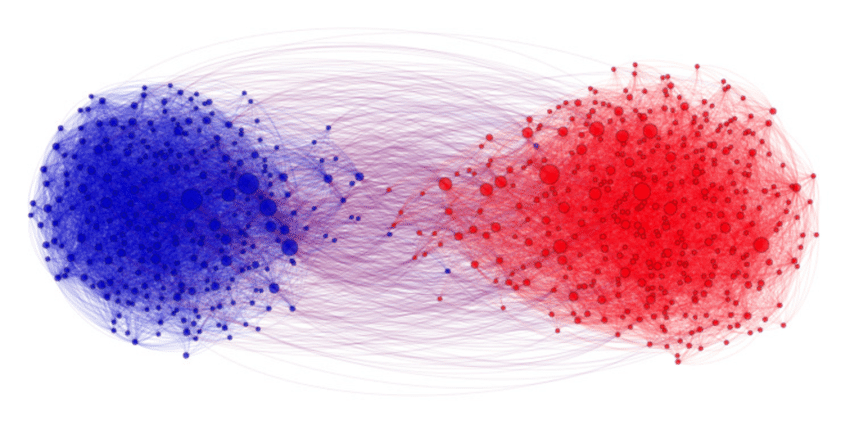
\includegraphics[width=\textwidth]{png/uvod.png}
    % add footnote
    \begin{tiny}
        Izvor: Interian, Ruben i Ribeiro, Celso. (2018). An empirical investigation of network polarization. Applied Mathematics and Computation. 339. 651-662. 10.1016/j.amc.2018.07.066.
    \end{tiny}
\end{frame}

\begin{frame}
	\frametitle{Ugrađivanje (embedovanje) čvorova}
	Neka je $ G = (V, E) $ graf, tada je ugrađivanje (embedovanje) funkcija 

	$$ U : V \to \mathbb{R}^n $$ 

	koja preslikava čvorove grafa u n-dimenzionalni euklidski prostor tako da čvorovi koji su dosta međusobno povezani budu blizu po euklidskom rastojanju
	

\end{frame}

\begin{frame}{node2vec algoritam}
	\centering
    \begin{tikzpicture}[node distance=2cm]

    % Blokovi
    \node (walks) [block] {Slučajne šetnje po čvorovima grafa};
    \node (embedding) [block, below of=walks] {Ugrađivanje (Embedding)};

    % Strelice
    \draw [arrow] (walks) -- (embedding);

    \end{tikzpicture}
\end{frame}

\begin{frame}{Ciljevi istraživanja}
    \begin{itemize}
        \item Implementacija paralelne verzije node2vec algoritma
        \item Analiza ubrzanja u odnosu na serijsku verziju na klasteru sa više čvorova
        \item Analiza kvaliteta dobijenog ugrađivanja
    \end{itemize}
\end{frame}


\section{Arhitektura}
\begin{frame}{Arhitektura}
    \centering
    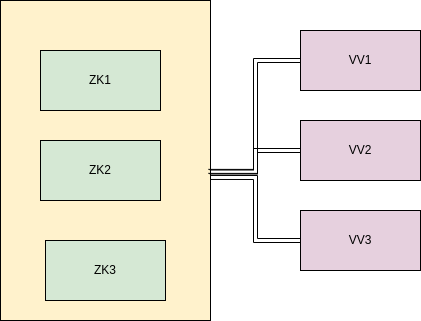
\includegraphics[height=0.8\textheight]{./png/Arhitektura i infrastruktura.drawio.png}
\end{frame}

\begin{frame}{Način rada - master i radni čvorovi}
    \begin{columns}
        \begin{column}{0.5\textwidth}
            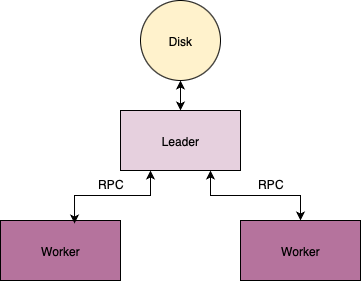
\includegraphics[height=0.5\textheight]{./png/Classic mode.drawio.png}
    \end{column}
    \begin{column}{0.5\textwidth}
        \begin{itemize}
            \item Master čvor:
            \begin{itemize}
                \item Učitava graf iz baze podataka
                \item Particioniše graf
                \item Raspoređuje particije po radnim čvorovima
                \item Prikuplja rezultate od radnih čvorova
                \item Spaja rezultate u konačno ugrađivanje
            \end{itemize}
            \item Radni čvorovi:
            \begin{itemize}
                \item Učitavaju particiju grafa iz baze podataka
                \item Izvršavaju node2vec algoritam na učitanom delu grafa
                \item Šalju rezultate nazad master čvoru
            \end{itemize}
        \end{itemize}
    \end{column}
    \end{columns}
\end{frame}

\begin{frame}{Način rada - Deljeni resursi}
    \begin{columns}
        \begin{column}{0.5\textwidth}
            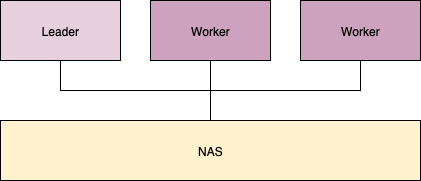
\includegraphics[width=0.5\textheight]{./png/NAS mode.drawio.png}
        \end{column}
        \begin{column}{0.5\textwidth}
            \begin{itemize}
                \item Izabere se jedan glavni čvor koji radi koordinaciju zadataka.
                \item Koordinator prosleđuje reference ka particijama
                \item Svi procesi imaju deljeno skladište za podatke
                \item Značajno pogodnije da se koristi sa integracijom sa SLURM-om.
            \end{itemize}
        \end{column}
    \end{columns}
\end{frame}

\section{Blokovski prikaz algoritma}
\begin{frame}{Blokovski prikaz algoritma}
    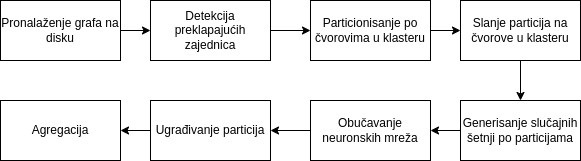
\includegraphics[width=\textwidth]{./png/Blokovski prikaz algoritma.drawio.png}
\end{frame}

\section{Particionisanje}
\begin{frame}{Detekcija preklapajućih zajednica}
    \begin{itemize}
        \item Algoritam za detekciju preklapajućih zajednica 
        \item Za svaki čvor koji nije dodeljen zajednici, dodeljuje se nova zajednica 
        \item Dodaju se susedni čvorovi čvorova u zajednici čije dodavanje uvećava kvalitet zajednice po funkciji $ f = \frac{k_\text{in}}{(k_\text{out} + k_\text{in})^\alpha} $ 
        \item Nakon dodavanja, uklanjaju se čvorovi čije uklanjanje povećava kvalitet zajednice
        \item Postupak se ponavlja sve dok postoje čvorovi koji nisu dodeljeni nekoj zajednici
    \end{itemize}
\end{frame}

\begin{frame}{Detekcija preklapajućih zajednica - modifikacija algoritma}
    \begin{itemize}
        \item Zbog povećanja brzine, algoritam se modifikuje tako da ne traje sve dok postoje čvorovi koji nisu dodeljeni zajednici
        \item Umesto toga, algoritam se izvršava dok određeni broj čvorova nije dodeljen zajednici
    \end{itemize}
\end{frame}

\begin{frame}{Particionisanje po čvorovima u klasteru}
    \begin{itemize}
        \item Nakon detekcije zajednica, potrebno je rasporediti zajednice po čvorovima u klasteru
        \item U ovom radu, korišćen je bin packing algoritam
        \item Algoritam raspoređuje zajednice po čvorovima, tako da čvorovi u klasteru budu što sličniji po svom opterećenju
        \item Opterećenje čvora K, kom su raspoređene zajednice $ S_K $, je $ \sum_{s \in S_K} |s| $
        \item Težine se zatim sortiraju u opadajućem redosledu, počevši od najveće.
        \item Inicijalno, maksimalna veličina (kapacitet) particije je prosečna veličina zajednice 
    \end{itemize}
\end{frame}

\begin{frame}
    \frametitle{Particionisanje po čvorovima u klasteru}
    \begin{itemize}
        \item Algoritam dodeljuje particije zajednicama, počevši od najveće zajednice. Uvek se dodeljuje particija koja je najmanje opterećena
        \item Ukoliko ne postoji particija koja ima potreban kapacitet, kapacitet particija se povećava za prosečnu veličinu zajednice koja još nije dodeljena particiji. 
        \item Ovaj proces se ponavlja dok sve zajednice ne budu raspoređene.
    \end{itemize}
\end{frame}




\section{Korišćeni skupovi podataka}
\begin{frame}{Skupovi podataka}
    \begin{itemize}
        \item Poznati grafovi iz literature 
        \begin{itemize}
            \item Zaharijev karate klub
            \item Les Miserables
            \item Davis southern women
            \item Florentine families
        \end{itemize}
        \item Twitch mreža
        \item Sintetički grafovi 
    \end{itemize}
\end{frame}

\section{SLURM job scheduler}
\begin{frame}{SLURM job scheduler}
    \begin{itemize}
        \item SLURM (Simple Linux Utility for Resource Management) je open-source sistem za upravljanje resursima i raspoređivanje poslova na klasterima.
        \item Omogućava korisnicima da lako podnesu, upravljaju i prate svoje poslove na klasteru.
        \item SLURM podržava različite strategije raspoređivanja, uključujući FIFO, priority-based i backfill.
    \end{itemize}
\end{frame}

\begin{frame}{SLURM i VertexVoyage}
    \begin{itemize}
        \item VertexVoyage može interagovati sa SLURM-om
        \item VertexVoyage dobija informacije o trenutnom zadatku na osnovu promenljivih okruženja koje postavlja SLURM
        \item Dva moda pokretanja:
        \begin{itemize}
            \item Pokretanje N poslova gde je jedan master 
            \item Ručno pokretanje poslova za ugrađivanje nakon particionisanja
        \end{itemize}
    \end{itemize}
\end{frame}

\begin{frame}{Ubrzanje}
\begin{itemize}
    \item Ubrzanje (engl. speedup) je mera koliko je paralelni algoritam brži u odnosu na serijski algoritam
    \item Definisano kao:
    $$ S = \frac{T_1}{T_p} $$
    gde je $ T_1 $ vreme izvršavanja serijskog algoritma, a $ T_p $ vreme izvršavanja paralelnog algoritma na $ p $ procesora (čvorova na klasteru)
    \item Opseg se definiše kao:
    $$ R = \frac{T_1}{T_\infty} $$
    gde je $ T_\infty $ vreme izvršavanja paralelnog algoritma sa beskonačnim brojem procesora
    \item Idealno ubrzanje je linearno, tj. $ S = p $
    \item U praksi, zbog režijskih troškova komunikacije i sinhronizacije, ubrzanje je često manje od idealnog
\end{itemize}
\end{frame}

\begin{frame}
\begin{itemize}
    \item Amdahlov zakon daje gornju granicu ubrzanja:
    $$ S \leq \frac{1}{f + \frac{1-f}{p}} $$
    gde je $ f $ frakcija serijskog dela algoritma u odnosu na Ukupno vreme izvršavanja.
    \item Neka je $T_{\text{part}}$ vreme particionisanja, a $T_{\text{embed}}(i)$ vreme ugrađivanja na čvoru $i$. Tada je ukupno vreme izvršavanja paralelnog algoritma:
    $$ T_p = T_{\text{part}} + \max_{i=1}^{p} T_{\text{embed}}(i) $$
    \item Ukupno vreme izvršavanja serijskog algoritma (koji ne zahteva particionisanje) je:
    \item $$ T_1 = \sum_{i=1}^{K} T_{\text{embed}}(i) $$
\end{itemize}    
\end{frame}

\section{Rezultati}
\begin{frame}{Vreme particionisanja za realne mreže iz literature i Twitch}
    \centering
    \begin{table}
        \label{tab:4.2}
        \begin{tabular}{p{1.4in}p{1in}p{0.5in}p{0.5in}}
        Mreža & Vreme particionisanja (s)& Broj čvorova & Broj grana \\
        \hline
        Zaharijev karate klub & 0.001 & 34 & 78 \\
        Les Mis & 0.004 & 77 & 254 \\
        Davis southern women & 0.004 & 32 & 89 \\
        Florentine families & 0.0006 & 15 & 20 \\
        Twitch  & 1638.00 & 168114 & 6797557 \\
    \end{tabular}
\end{table}
\end{frame}
    
\begin{frame}{Vreme particionisanja za sintetički graf}
    \centering
    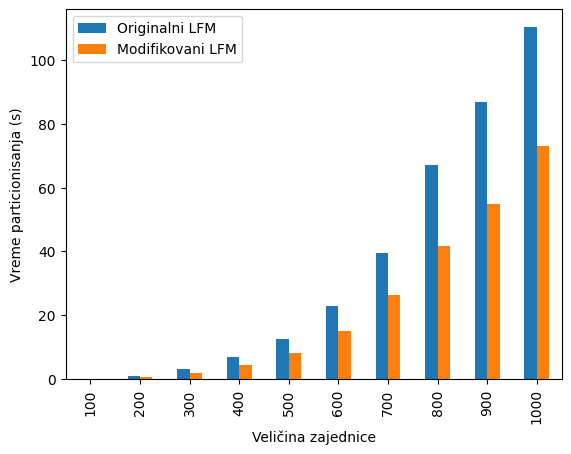
\includegraphics[height=0.8\textheight]{csv/4.3.png}
\end{frame}

\begin{frame}
    \frametitle{Ukupno vreme ugrađivanja na sintetičkom grafu}
    \centering
    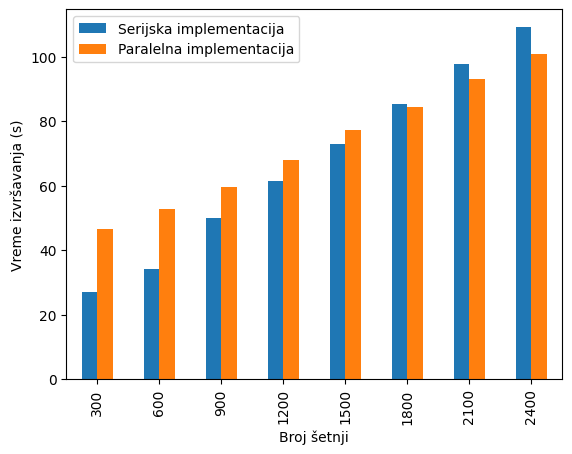
\includegraphics[height=0.8\textheight]{csv/4.13.png}
\end{frame}

\begin{frame}{Rezultati - vreme ugrađivanja na SBM sa 10M ivica}
    \begin{table}
    \caption{Uporedna analiza performansi za LFM algoritam particionisanja}
    \label{tab:Performance_comparison_max_Node2Vec_vs_modified__lfm_on_SBM_10M_with_varying_threshold}
    \begin{tabular}{p{1in}p{1in}p{1in}p{1in}}
    \hline 
    & Vreme particionisanja & Vreme ugrađivanja na 16 & Vreme ugrađivanja na 1 \\
    Prag &  &  &  \\
    \hline
    0.000000 & 14118.587150 & 90.071612 & 174.646026 \\
    0.500000 & 12948.078974 & 82.932776 & 158.931893 \\
    1.000000 & 0.005604 & 60.919978 & 925.772633 \\
    \hline
    \end{tabular}
    \end{table}
    
\end{frame}

\begin{frame}
\begin{table}
\caption{Uporedna analiza performansi za LFM algoritam particionisanja}
\label{tab:Performance_comparison_max_Node2Vec_vs_modified__lfm_on_SBM_10M_with_varying_alpha}
\begin{tabular}{p{1in}p{1in}p{1in}p{1in}}
\hline
 & Vreme particionisanja & Vreme ugrađivanja na 16 & Vreme ugrađivanja na 1 \\
Alpha parametar &  &  &  \\
\hline
1.000000 & 15151.445818 & 96.892017 & 188.360206 \\
1.500000 & 14384.355827 & 83.339856 & 161.653478 \\
2.000000 & 1489.028646 & 60.098522 & 14927.836920 \\
\hline
\end{tabular}
\end{table}
    
\end{frame}

\begin{frame}
\begin{table}
    
\caption{Uporedna analiza performansi za LFM algoritam particionisanja}
\label{tab:Performance_comparison_max_Node2Vec_vs_lfm_on_SBM_10M_with_varying_partition_num}
\begin{tabular}{p{1in}p{1in}p{1in}p{1in}}
\hline
 & Vreme particionisanja & Paralelna implementacija & Sekvencijalna implementacija \\
Broj particija &  &  &  \\
\hline
1 & 77.875600 & 107.061880 & 107.061880 \\
2 & 155.384691 & 102.909459 & 198.506485 \\
4 & 318.065973 & 90.397061 & 360.115173 \\
8 & 604.270801 & 107.493993 & 724.160440 \\
16 & 1202.096511 & 113.680622 & 1407.603405 \\
32 & 2384.997995 & 122.427380 & 2801.377654 \\
\hline
\end{tabular}
\end{table}
\end{frame}

\section{Zaključak}
\begin{frame}{Zaključak}
    \begin{itemize}
        \item Pokazano je da:
        \begin{itemize}
            \item Paralelna implementacija algoritma jeste brža od serijske, nakon određenog broja šetnji, dok zadržava kvalitet rekonstrukcije grafa
            \item Klasterovanje dobijeno paralelnim ugrađivanjem jeste slično klasterovanju dobijenom serijskim ugrađivanjem
        \end{itemize}
        \item \textbf{Predloženi metod se može koristiti da ubrza ugrađivanje čvorova ili da, uz dodatno vreme particionisanja, uveća tačnost zbog većeg broja mogućih slučajnih šetnji}
        \item Unapređenja:
        \begin{itemize}
            \item Upotreba specifične baze podataka koja bi indeksirala čvorove tako da particionisanje bude brže
            \item Poređenje paralelne i serijske implementacije na drugim primenama
            \item fino podešavanje parametara modela za velike mreže 
        \end{itemize}
    \end{itemize}
\end{frame}



\begin{frame}
	\begin{center}
		\Huge Hvala na pažnji!
	\end{center}
\end{frame}


\end{document}
